\documentclass[border=1cm]{standalone}
\usepackage{tikz}
\begin{document}

\begin{tikzpicture}
\draw (-1,0)-- (3,10pt)-- (35:3);
\end{tikzpicture}

\begin{tikzpicture}
\draw[->] (-1,0)-| (3,10pt);
\draw[red] (3,10pt)-- (35:3);
\end{tikzpicture}

\begin{tikzpicture}
\draw (-1,0) to (5,1);
\draw[green] (-1,0) to[out=90,in=135] (5,1);
\draw[cyan] (-1,0) .. controls (0,-2) .. (5,1);
\end{tikzpicture}

\begin{tikzpicture}
\draw[dotted,gray] (-1,0)-- (5,1);
\draw (-1,0) .. controls (0,-2) and (4,2) .. (5,1);
\end{tikzpicture}

\begin{tikzpicture}[scale=3]
\draw (0,0) node {hello}-- (1,1) node {world};
\end{tikzpicture}

\begin{tikzpicture}[scale=3]
\draw (0,0)-- (1,1) node[midway]{A} node[pos=0.75,above]{B} node[right]{C};
\end{tikzpicture}

\begin{tikzpicture}[scale=3]
\draw (0,0) to node[midway]{A} node[pos=0.75, above]{B} (1,1) node[right]{C};
\end{tikzpicture}

\begin{tikzpicture}[scale=3]
\draw (0,0) node[circle, draw]{$\sum_{i=1}^{n}n^2$}-- (1,1)
node[rectangle,draw]{$\frac{1}{\sqrt{2}}$};
\end{tikzpicture}

\begin{tikzpicture}[scale=3]
% define nodes
\node[circle,draw] (label1) at (0,0) {$\sum_{i=1}^{n}n^2$};
\node[rectangle,draw] (label2) at (1,1) {$\frac{1}{\sqrt{2}}$};
% draw the line
\draw (label1)-- (label2);
\end{tikzpicture}

\begin{tikzpicture}[scale=2]
  % Define the nodes
\node[circle, draw] at (0,0) (a) {A};
\node[rectangle, fill] at (3,0) (b) {};
\node at (3,0.4) (blabel) {B};
\node[rectangle,rounded corners, draw] at (5,2) (c) {C};
% Draw the paths
\draw[->, green] (a)-- (b) node[midway, below,black]{2};
\draw[<->, blue] (a) to[out=45, in=135] (b);
\draw[->>,red] (b)--(c);
\draw[yellow,dotted,very thick] (b) |- (c);
\draw[<-,cyan] (b)-| (c);
\draw[thick,black] (a).. controls (1,5) .. (c) node[midway,above]{$\frac{1}{2}$};
\end{tikzpicture}

\begin{tikzpicture}
\draw [domain=-2:2] plot (\x, {pow(\x,2});
\end{tikzpicture}

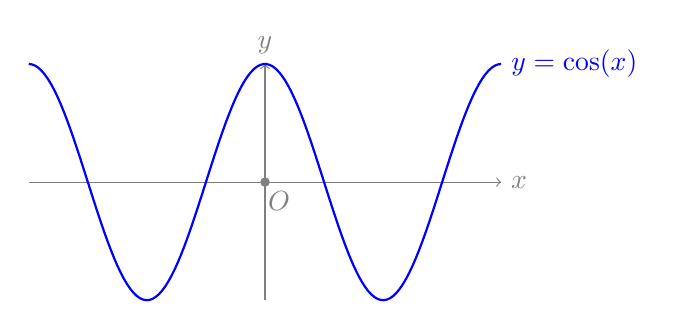
\begin{tikzpicture}[scale=1.5]
% Draw the x and y axis, label the axes and the origin
\draw[gray,->] (-2,0)-- (2,0) node[right]{$x$} node[pos=0.53, below]{$O$};
\draw[gray,->] (0,-1)-- (0,1) node[above]{$y$};
\draw[fill,gray] (0,0) circle [radius=1pt];
% Plot the curve
\draw[blue, thick] [domain=-2:2, samples=150] plot (\x, {cos(pi*\x r)})
node[right]{$y = \cos(x)$};
% Note: the r in the argument of the cosine signifies that we enter \x in radians
\end{tikzpicture}

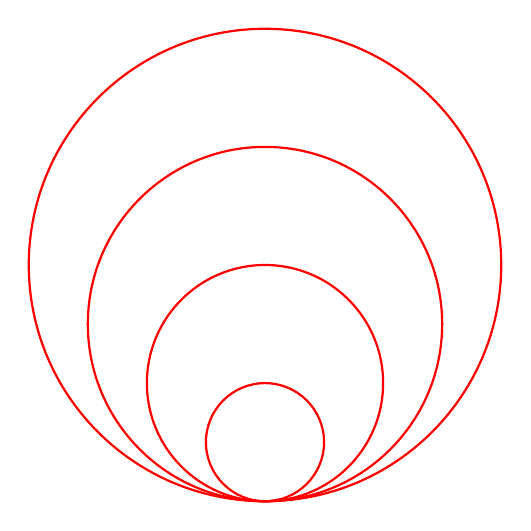
\begin{tikzpicture}[scale=0.75]
\foreach \x in {0,1,2,3}
\draw[red,thick] (0,\x) circle [radius=\x+1];
\end{tikzpicture}

\end{document}